\section{Introduction} \label{sec:intro}
%The next line produces an indented paragraph to start the document
 %unit.  The LaTeX defaults start most units without indentations.
\hspace{\parindent}

Ten years after the discovery of the proton by Rutherford in
1920~\cite{Rutherford:1920}, Pauli postulated ``a particle that cannot be
detected" which later became known as the neutrino. The neutrino was eventually
detected by Reines and Cowan in 1956~\cite{Reines:1956rs}.  Our understanding
of both the proton and the neutrino has radically changed since they were
discovered. In the 1960s Gell-Mann and Zweig independently proposed that proton
had an internal structure composed of a new particle called
quarks~\cite{GellMann:1964nj,Zweig:1981pd,Zweig:1964jf}.  This quark
substructure was first detected in 1968 at the Stanford Linear Accelerator
Lab~\cite{Friedman:1972sy}. Also in 1968, Davis built a detector to measure
neutrinos coming from the sun and detected fewer than predicted by
theory~\cite{Davis:1968cp,Bahcall:1968hc}. This was later confirmed in 1998 by
the Super-Kamiokande collaboration~\cite{Fukuda:1998mi} to be because neutrinos
are able to oscillate into other flavors, violating lepton number conservation.

Two decades later in 1987, the European Muon Collaboration (EMC) discovered
that the spin of the quarks in the proton only add up to a small percentage of
the total spin of the proton~\cite{Ashman:1987hv}, referred to as the proton spin puzzle. In
addition to the total quark spin contribution being smaller than expected, the
EMC also saw evidence that the net spin contribution from the strange
quark-antiquark pairs in the proton's quark-gluon sea was not zero as expected
but actually negative\cite{Ashman:1989ig}.

In 1997 the Liquid Scintillator Neutrino Detector (LSND) collaboration
announced that it had observed an anomaly in the neutrino oscillation
spectrum~\cite{Aguilar:2001ty} which might suggest a fourth generation of
neutrinos that do not interact via the standard model, called sterile
neutrinos. This announcement led to the MiniBooNE experiment which was unable
to verify the LSND anomaly, but observed a new anomaly at low neutrino
energy~\cite{Aguilar-Arevalo:2010wv,Aguilar-Arevalo:2018gpe}, known as the low
energy excess, which may also suggest sterile neutrinos.

The MicroBooNE experiment~\cite{Acciarri:2016smi} was designed to be able to
investigate the MiniBooNE low energy excess. Interestingly, the design
parameters required to allow MicroBooNE to shed light on the MiniBooNE excess
happen to make it an ideal experiment for studying the mystery of strange quark
spin structure in the proton that was found by the EMC.


%%%%%%%%%%%%%%%%%%%%%%%%%%%%%%%%%%%%%%%%%%%%%%%%%%%%%%%%%%%
% Standard Model
%%%%%%%%%%%%%%%%%%%%%%%%%%%%%%%%%%%%%%%%%%%%%%%%%%%%%%%%%%%
\subsection{The Standard Model}\label{sec:standardmodel}

The standard model of particle physics, illustrated in
Fig.~\ref{fig:standardmodel}, classifies all of the known elementary particles
and describes the fundamental forces between them. The elementary particles in
the standard model are divided into the particles with half-integer spin called
fermions that make up matter and the particles with whole-integer spin called
bosons that carry the forces between particles.
\begin{figure}
  \centering
  \includegraphics[angle=0,width=3.5in]{figures/intro/Standard_Model_of_Elementary_Particles.png}
  \caption{The standard model of particle physics taken from~\cite{MissMJ}.}
  \label{fig:standardmodel}
\end{figure}

The fermions are further divided based on what type of forces they interact
with.  The six quarks (and six antiquarks) can interact via all three standard
model forces. The quarks compose protons and neutrons and are the only fermions
that can interact via the strong force. The six leptons (and six anti-leptons)
can all interact via the weak force, and the charged leptons (electrons, muons,
and tau leptons) can interact via the electromagnetic force, but the neutral
neutrinos cannot. The quarks and leptons are also divided into three
``generations", also illustrated in Fig.~\ref{fig:standardmodel}. Almost all
matter is composed of the first generation fermions which includes electrons
and up and down quarks.

The bosons consist of the gluon which carries the strong force, the photon
which carries the electromagnetic force, the W$^{\pm}$ and Z$^0$ bosons which
carry the weak force, and the Higgs boson which gives the particles their mass.
As their names suggest, the strong force is much stronger than the other
forces, and the weak force is the weakest force in the standard model, and the
electromagnetic force is in between.

It is due to the fact that neutrinos can only interact via the weakest force
that makes them so difficult to detect. The probability of a given neutrino
interacting with any other particle is very low. This is also what allows us to
use neutrinos to probe the internal quark and gluon structure of protons and
neutrons.

%%%%%%%%%%%%%%%%%%%%%%%%%%%%%%%%%%%%%%%%%%%%%%%%%%%%%%%%%%%
% Spin Structure of Nucleons
%%%%%%%%%%%%%%%%%%%%%%%%%%%%%%%%%%%%%%%%%%%%%%%%%%%%%%%%%%%
\subsection{The Spin Structure of Nucleons} \label{sec:nuctheory}
  Protons and neutrons, called nucleons, are composed of three up and down
  quarks and the gluons that bind the quarks together. These gluons carry
  enough energy to split into short-lived quark-antiquark pairs inside the
  nucleon making up a quark-gluon sea. The sea is made up of gluons and up,
  down, and strange quarks and antiquarks. The momentum, electromagnetic, and
  spin structure of each component of the quark-gluon sea is an active area of
  research.

  \subsubsection{Spin Structure Functions}
  In inclusive lepton-nucleon deep inelastic scattering (DIS), it is useful to
  parameterize the scattering cross section in terms of nucleon structure
  functions $F_1(x)$, $F_2(x)$, $g_1(x)$, and $g_2(x)$. In the QCD parton
  model~\cite{Feynman:1969wa}, $x$ is the fraction of the nucleon's momentum
  carried by the quarks, and $g_1$ and $g_2$, the spin structure functions,
  parameterize the polarized DIS cross section~\cite{Thomas:2001kw}.

  The $g_1$ spin structure function can be written as a combination of the spin
  contribution from each of the quark flavors~\cite{Bass:2007zzb},
  \begin{equation}
    g_1(x) = \frac{1}{2}\sum_q e_q^2 \Delta q(x) \,,
  \end{equation}
  where $q$ is the quark flavor ($q = u,d,s$), $e_q$ is the electric charge of
  the quark, and $\Delta q$ is the contribution of the quark spin to the
  nucleon spin,
  \begin{equation}
    \Delta q(x) = \big(q^{\uparrow} + \bar{q}^{\uparrow}\big)(x) 
      - \big(q^{\downarrow} + \bar{q}^{\downarrow}\big)(x) \,.
  \end{equation}
  Here $q^{\uparrow}(x)$ \big($q^{\downarrow}(x)$\big) is the probability of
  finding a quark with momentum fraction $x$ with its spin in the same
  (opposite) direction of the nucleon's spin, and $\bar{q}^{\uparrow}(x)$
  \big($\bar{q}^{\downarrow}(x)$\big) is the probability of finding an
  antiquark with momentum fraction $x$ with its spin in the same (opposite)
  direction of the nucleon's spin. Integrating over the quark spin structure
  gives the net quark spin contribution to the nucleon spin
  \begin{equation}
    \Delta q = \int_0^1 \Big[\big(q^{\uparrow} + \bar{q}^{\uparrow}\big)(x)
      - \big(q^{\downarrow} + \bar{q}^{\downarrow}\big)(x) \Big] dx \,.
  \end{equation}

  \subsubsection{The Ellis-Jaffe Sum Rule}

  The Ellis-Jaffe sum rule~\cite{Ellis:1973kp} relates the integral of the
  $g_1$ spin structure function to the axial charges~\cite{Thomas:2001kw},
  \begin{align}
    g_A &= \Delta u - \Delta d \\
    g_A^{(8)} &= \Delta u + \Delta d - 2\Delta s \\
    g_A^{(0)} &= \Delta u + \Delta d + \Delta s \,.
  \end{align}
  where $g_A$ is the isovector axial charge, $g_A^{(8)}$ is the $SU(3)$ octet
  axial charge, and $g_A^{(0)}$ is the flavor-singlet axial charge. For the
  proton, the integral of the $g_1$ spin structure function is
  \begin{equation}
    \begin{aligned}
    S_p &= \int_0^1 dx g_{1p}(x)  \\
        &= \int_0^1 dx \Big[\frac{4}{18}\Delta u(x) 
        + \frac{1}{18} \Delta d(x) + \frac{1}{18} \Delta s(x) \Big] \,, \\
        &= \frac{4}{18}\Delta u + \frac{1}{18}\Delta d + \frac{1}{18}\Delta s \,, \\
        &= \frac{g_A}{12} + \frac{g_A^{(8)}}{38} + \frac{g_A^{(0)}}{9} \,.
    \end{aligned}
  \end{equation}
  The axial charges can be determined through experimental measurements.  The
  isovector axial charge, $g_A$, can be obtained in neutron
  $\beta$-decay~\cite{Dubbers:1991bh}. Assuming $SU(3)$ symmetry, $g_A^{(8)}$
  can be obtained though hyperon $\beta$-decay. If the net strange contribution
  to the nucleon spin is assumed to be negligible, the flavor-singlet charge is
  equal to the $SU(3)$ octet charge,
  \begin{equation}
     \Delta s \sim 0 \Rightarrow g_A^{(0)} = g_A^{(8)} \,.
  \end{equation}

  \subsubsection{Experimental Tests of the Ellis-Jaffe Sum Rule}
  One of the first experiments to test the Ellis-Jaffe sum rule through
  inclusive DIS was the European Muon Collaboration (EMC) at CERN in
  1989~\cite{Ashman:1987hv,Ashman:1989ig}. The EMC scattered polarized muons
  off a polarized proton target and detected the scattered muon in a forward
  muon spectrometer. Figure~\ref{fig:emcej} shows the EMC measurement of the
  integral of the $g_1$ spin structure function as a function of the lower
  bound on the integral, $x_m$, and the expected value of the integral at $x_m
  = 0$ from the Ellis-Jaffe sum rule. There is a significant discrepancy
  between the measured value and the value expected from theory. Assuming that
  the discrepancy comes from the assumption that $\Delta s = 0$, and not the
  $SU(3)$ symmetry assumption, the extracted non-zero value of $\Delta s$ to
  resolve the difference is
  \begin{equation}
    \Delta s_{\textrm{EMC}} = -0.095 \pm 0.016 \pm 0.023 \,.
  \end{equation}
  This implies not only that the overall spin polarization of the strange
  quarks and antiquarks in the nucleon sea is nonzero, but that they are
  polarized in the opposite direction of the proton.
  \begin{figure}[h]
    \centering
    \includegraphics[angle=0,width=5.5in]{figures/intro/strfunctions/EMC_Ellis-Jaffe.png}
    \caption{The integral of the $g_1(x)$ spin structure function measured by
      the EMC experiment~\cite{Ashman:1989ig}.}
    \label{fig:emcej}
  \end{figure}

  After the EMC result, many subsequent polarized target inclusive DIS
  experiments tested the Ellis-Jaffe sum rule over the next few decades.
  See Refs.~\cite{Aidala:2012mv}~and~\cite{Bass:2007zzb} for detailed reviews.
  Several inclusive DIS polarized target experiments were performed at
  SLAC~\cite{Baum:1983ha,Anthony:1996mw,Abe:1998wq} with a polarized electron
  beam, at CERN with the polarized muon beam by the Spin Muon Collaboration
  (SMC)~\cite{Adeva:1993km,Adeva:1998vv} and by
  COMPASS~\cite{Alexakhin:2006oza}, the polarized electron or positron HERA
  beam at DESY by the
  HERMES~\cite{Ackerstaff:1997ws,Ackerstaff:1999ey,Airapetian:2006vy}
  collaboration. A more recent measurements of the violation of the Ellis-Jaffe
  sum rule from polarized muon inclusive DIS off a polarized target in the
  COMPASS experiment in 2007 gives~\cite{Alexakhin:2006oza} $\Delta
  s_{\textrm{COMPASS}} = -0.08 \pm 0.01 \pm 0.02$, and from the HERMES
  experiment in 2007 gives~\cite{Airapetian:2006vy} $\Delta s_{\textrm{HERMES}}
  = -0.085 \pm 0.013 \pm 0.008 \pm 0.009$.

  The nucleon spin structure can also be studied through semi-inclusive deep
  inelastic scattering (SIDIS). In SIDIS, in addition to detecting the
  scattered lepton, at least one of the final state pions or kaons is detected.
  If the detected hadron has a large enough fraction of the energy transfer, it
  can be assumed that it contains the quark that was struck by the
  lepton~\cite{Bass:2007zzb}.  A factor is included in the measured spin
  structure functions that describes the probability of a struck quark
  producing a pion or kaon with the measured energy fraction. This factor is
  called a fragmentation function, and it can be used to reconstruct individual
  quark flavor contributions to the nucleon spin. Several experiments have made
  measurements of the strange quark spin through SIDIS including
  COMPASS~\cite{Alekseev:2009ac,Alekseev:2010ub} at CERN and
  HERMES~\cite{Airapetian:2003ct,Airapetian:2004zf,Airapetian:2008qf} at DESY.
  Measurements of the strange quark polarization in the nucleon through SIDIS
  tend to favor much smaller values of $\Delta s$ that are consistent with
  zero. While these results depend less on $SU(3)$ flavor symmetry than
  inclusive DIS results, they do depend strongly on the choice of fragmentation
  functions. Results from global analyses of both DIS and SIDIS
  data~\cite{deFlorian:2008mr,deFlorian:2009vb,Blumlein:2010rn,Nocera:2014gqa,Leader:2014uua}
  tend to give negative values of $\Delta s$.
  
  In addition to the experimental effort, there has been a parallel effort to
  calculate the standard model prediction of the nucleon structure using
  lattice QCD. Early lattice QCD calculations of $\Delta
  s$~\cite{Savage:1996zd,Dong:1995rx} suggested negative values at a similar
  scale to what is measured in inclusive DIS. The value found
  in Ref.~\cite{Dong:1995rx} was $\Delta s = -0.12 \pm 0.01$. More recent
  calculations~\cite{QCDSF:2011aa,Engelhardt:2012gd,Abdel-Rehim:2015lha,Chambers:2015bka}
  give results of $\Delta s$ much closer to zero, but still negative. The newer
  results are more similar to the values measured in SIDIS. For example,
  $\Delta s = -0.031 \pm 0.017$ was found in Ref.~\cite{Engelhardt:2012gd} and
  $\Delta s = - 0.018 \pm 0.006$ was found in Ref.~\cite{Chambers:2015bka}.


%%%%%%%%%%%%%%%%%%%%%%%%%%%%%%%%%%%%%%%%%%%%%%%%%%%%%%%%%%%
% Neutrinos as a Nucleon Probe
%%%%%%%%%%%%%%%%%%%%%%%%%%%%%%%%%%%%%%%%%%%%%%%%%%%%%%%%%%%

\subsection{Neutrino Measurements of the Strange Spin Structure}
\label{sec:neutrinos}
  Since neutrinos only interact via the weak force, neutrino-nucleon elastic
  scattering is sensitive to the weak currents and are great tools for
  measuring the axial form factor, $G_A(Q^2)$.
  See Refs.~\cite{Lyubushkin:2008pe}~and~\cite{Formaggio:2013kya} for detailed
  reviews of the many measurements of $G_A(Q^2)$ through charged current
  quasi-elastic (CCQE) scattering. Neutral current (NC) elastic
  neutrino-nucleon scattering ($\nu N \rightarrow \nu N$) specifically is
  sensitive to the NC form factor $G_A^{NC}(Q^2)$ which contains
  contributions from the up, down, and strange quarks to the spin structure
  of the nucleon ($G_A(Q^2)$ only contains contribution from the up and down
  quarks).

  At the limit where the negative four-momentum transfer squared, $Q^2$, goes
  to zero, the NC axial form factor becomes a combination of the net spin
  contribution from each of the quarks to the nucleon spin~\cite{Bass:2007zzb},
  \begin{equation}
    G_A^{NC}(Q^2 = 0) = \frac{1}{2}(\Delta u - \Delta d - \Delta s)
  \end{equation}

  The reconstructed $Q^2$ is determined entirely from the recoil nucleon
  kinetic energy using
  \begin{equation}
    \begin{aligned}
    Q^2_N &= -q^2 = -(p'_N - p_N)^2 \\
          &= -(E'_N - E_N)^2 + (\bf{p}'_N - \bf{p}_N)^2 \\
          &= 2 T_N M_N,
    \end{aligned}
  \end{equation}
  where $p$ is four-momentum, $E$ is energy, $\bf{p}$ is three-momentum, $M$ is
  mass, $T$ is kinetic energy determined by the length of the track, the $N$
  subscript represents the nucleon in the neutrino-nucleon interaction, the
  prime represents the final state, and the nucleon momentum in the nucleus is
  assumed to be small compared to the final nucleon momentum. This means that
  the ability to measure the axial form factor at low $Q^2$ in NC elastic
  neutrino-nucleon scattering depends on the experimental nucleon energy
  threshold.

  Two previous neutrino experiments have performed a measurement of $\Delta
  s$ through neutral current elastic neutrino-nucleon scattering. The first
  was the E734 experiment~\cite{Ahrens:1986xe} at Brookhaven National Lab (BNL) in
  1987, and the second was the MiniBooNE experiment~\cite{Aguilar-Arevalo:2010cx} at
  Fermilab in 2010.

  \subsubsection{The BNL E734 Experiment}\label{sec:e734}
  The main target and detector of the E734 experiment was 170~tons and was made
  of a combination of liquid scintillator cells and proportional drift tubes
  (PDTs). The liquid scintillator composed 80\% of the target and was used for
  calorimetry and timing, while the PDTs were used for position information.
  Additionally, there was a electromagnetic shower counter and a muon
  spectrometer just downstream of the main detector. The full detector
  schematic is shown in Fig.~\ref{fig:e734detector}.  The E734 detector sat in
  a neutrino beam at BNL that could run in either neutrino of antineutrino mode
  with a mean energy of 1.3~GeV for neutrino and 1.2~GeV for antineutrinos.
  Note that we are using natural units with the speed of light, $c$, set equal
  to one.
  \begin{figure}[h]
    \centering
    \includegraphics[angle=0,width=5.5in]{figures/intro/experiments/E734detector.pdf}
    \caption{Schematic of the BNL E734 detector~\cite{Ahrens:1986xe}.}
    \label{fig:e734detector}
  \end{figure}

  A simultaneous fit to the neutrino-proton and antineutrino-proton neutral
  current elastic cross sections in the range between $Q^2 = 0.45$~GeV$^2$ and
  $Q^2 = 1.05$~GeV$^2$ was performed to extract the neutral current axial form
  factor.  In the parameter estimation, the NC axial form factor was assumed to
  have the form
  \begin{equation}\label{eq:axdipole}
    G_A^{NC}(Q^2) = \frac{1}{2}\frac{g_A}{(1+Q^2/M_A^2)^2}(1+\eta) \,,
  \end{equation}
  where $g_A$ is the weak coupling constant, $M_A$ is the axial mass, and
  $\eta$ is a factor that encodes the difference between the charged current
  axial form factor and the strange axial form factor. This form assumes that
  both parts of the form factor have the exact same shape. If the difference is
  only due to the net spin contribution of the strange quark, $\Delta s$, then
  $\Delta s = -\eta g_A$ which was found to be $-0.15 \pm 0.09$ in this
  analysis. Figure~\ref{fig:e734xsec} shows the measured data and the cross
  section fits. Figure~\ref{fig:e734eta} shows the bounds on the axial mass
  $M_A$ and $\eta$ from the fit. 
  \begin{figure}[h]
    \centering
    \begin{subfigure}[t]{2.5in}
      \includegraphics[angle=0,width=2.5in]{figures/intro/experiments/E734flux.pdf}
      \caption{Measured neutrino-proton and antineutrino-proton cross sections.}
      \label{fig:e734xsec}
    \end{subfigure}
    \hspace{2pt}
    \begin{subfigure}[t]{2.5in}
      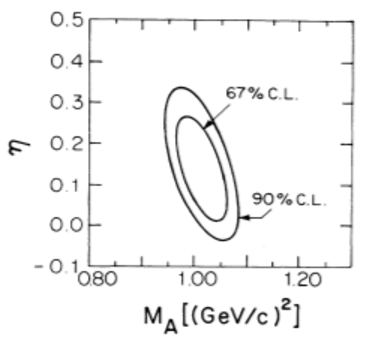
\includegraphics[angle=0,width=2.5in]{figures/intro/experiments/E734eta.pdf}
      \caption{Extracted neutral current axial form factor parameters.}
      \label{fig:e734eta}
    \end{subfigure}
    \caption{Results from the Brookhaven E734 measurement of the neutral
    current elastic cross section.}
    \label{fig:e734results}
  \end{figure}

  A later analysis of the E734 NC elastic data was
  performed~\cite{Garvey:1992cg} in which the strange part of the electric
  and magnetic form factors was not assumed to be zero. Four fits to the
  neutrino-proton and antineutrino-proton cross section data were performed.
  In the first fit, only the axial mass was allowed to vary and the strange
  quark contribution to the electric, magnetic, and axial form factors were
  all held fixed at zero. In the second, the strange contribution to the
  electric and magnetic form factors were fixed at zero, but the axial mass
  and the strange axial form factor were allowed to vary. In the third fit,
  all three strange form factors and the axial mass were allowed to vary, and
  in the last fit, the strange form factors were all allowed to vary, but the
  axial mass was held to the world average at the time, $M_A =
  1.032\pm0.036$~GeV. The same form of the axial form factor in
  Eq.~\ref{eq:axdipole} was assumed and the strange electric and magnetic
  form factors were assumed to have the same shape as the charged current
  electric and magnetic form factors. The extracted value of $\Delta s$
  ranged from $\Delta s = -0.13 \pm 0.09$ in the second fit to $\Delta s =
  -0.21 \pm 0.10$ in the fourth fit.  Each of the extracted $\Delta s$ values
  is consistent with the original measurement and with a $\Delta s$ being
  negative.  Additionally, a strong correlation between $\Delta s$ and $M_A$
  was again observed. In the first fit with $\Delta s$ fixed at zero, a best
  fit to the data was found when $M_A = 1.086 \pm 0.015$~GeV which is very
  consistent with the original results in Ref.~\cite{Ahrens:1986xe} shown in
  Fig.~\ref{fig:e734eta}.

  An additional analysis of the E734 data considering ratios of neutral
  current elastic interactions to charged current elastic interactions was
  performed~\cite{Alberico:1998qw}. Specifically, they looked at the
  neutrino-antineutrino asymmetry
  \begin{equation}
    \mathcal{A}_p(Q^2) = \frac{\Big(\frac{d\sigma}{dQ^2}\Big)_{\nu p \rightarrow \nu p} - \Big(\frac{d\sigma}{dQ^2}\Big)_{\bar{\nu} p \rightarrow \bar{\nu} p} }{\Big(\frac{d\sigma}{dQ^2}\Big)_{\nu n \rightarrow \mu^- p} - \Big(\frac{d\sigma}{dQ^2}\Big)_{\bar{\nu} p \rightarrow \mu^+ n}} \,.
  \end{equation}
  This asymmetry has an enhanced sensitivity to the strange axial and magnetic
  form factors. It was found that the experimental uncertainty was too large to
  determine $\Delta s$ and that a large factor of the uncertainty was due to
  the uncertainty on the axial mass. This analysis also assumed the dipole form
  of the axial form factor in Eq.~\ref{eq:axdipole}.

  A global analysis of the strange quark contribution to the electromagnetic
  and axial form factors performed in Ref.~\cite{Pate:2008va} included E734 NC
  elastic neutrino-proton scattering data. The analysis combined the E734 data
  with parity-violating elastic polarized-electron-proton scattering data from
  the G0~\cite{Armstrong:2005hs} and HAPPEx~\cite{Aniol:2004hp} experiments.
  The electron-proton data are sensitive to the strange contribution to the
  electric and magnetic form factors but not very sensitive to the strange
  axial form factor. The analysis found the extracted $\Delta s$ to be
  consistent with negative values.

  \subsubsection{The MiniBooNE Experiment}\label{sec:miniboonence}
  The main target and detector of the MiniBooNE experiment was 800 tons of
  scintillator oil in a 12.2~m diameter spherical tank. Charged particles
  from the neutrino interactions in the mineral oil produced Cerenkov light
  which was collected by 1520 8-inch PMTs surrounding the oil. A schematic of
  the detector is shown in Fig.~\ref{fig:miniboonedetector}.
  \begin{figure}[h]
    \centering
    \includegraphics[angle=0,width=4in]{figures/intro/experiments/miniboone.png}
    \caption{Schematic of the MiniBooNE detector~\cite{Cheng:2012yy}.}
    \label{fig:miniboonedetector}
  \end{figure}
  MiniBooNE sat in the Booster Neutrino Beam (BNB) at Fermilab that can run
  in either neutrino or antineutrino mode with an average neutrino energy of
  $\sim$800~MeV~\cite{Aguilar-Arevalo:2008yp}.

  The MiniBooNE collaboration performed a $\Delta s$ fit to the ratio of the
  neutrino-proton to the neutrino-nucleon NC elastic cross section in the
  proton kinetic energy between $T = 350$~MeV and $T = 800$~MeV. This
  corresponds to a range of $Q^2 = 0.66$~GeV$^2$ to $Q^2 = 1.5$~GeV$^2$.
  Figure~\ref{fig:miniboonedeltas} shows the measured ratio and the fits to the
  data.
  \begin{figure}[h]
    \centering
    \includegraphics[angle=0,width=4.5in]{figures/intro/experiments/miniboone_deltas.png}
    \caption{Ratio of the neutrino-proton NC elastic cross section to the
    neutrino-nucleon NC elastic cross section measured in
    MiniBooNE~\cite{Aguilar-Arevalo:2010cx}.}
    \label{fig:miniboonedeltas}
  \end{figure}
  In the analysis, the dipole shape in Eq.~\ref{eq:axdipole} was used for the
  axial form factor. When the value of the axial mass was held to $M_A =
  1.35$~GeV a value of $\Delta s = 0.08 \pm 0.26$ was found, and when the axial
  mass was held to $M_A = 1.23$~GeV a value of $\Delta s = 0.00 \pm 0.30$. Both
  of these values are consistent with the E734 measurement and with zero.

  A later analysis of the MiniBooNE data was performed which included a
  two-body current contribution to the cross section~\cite{Golan:2013jtj}.  The
  inclusion of the two-body current was done using the NuWro Monte Carlo
  neutrino event generator~\cite{Golan:2012wx}. The original MiniBooNE analysis
  used the NUANCE Monte Carlo neutrino event generator~\cite{Casper:2002sd}. A
  simultaneous extraction of $\Delta s$ and the axial mass from the asymmetry
  $\mathcal{A}_p(Q^2)$ assuming the dipole form of the axial form factor in
  Eq.~\ref{eq:axdipole} and including two-body currents resulted in an axial
  mass value of $M_A = 1.1^{+0.13}_{-0.15}$~GeV and $\Delta s =
  -0.4^{+0.5}_{-0.3}$. This result of $\Delta s$ is consistent both with the
  original MiniBooNE result and with zero.

  Very recently, another re-analysis of the MiniBooNE result was performed
  using updated lattice QCD calculations of the strange electric and magnetic
  form factors and the measured MiniBooNE NC elastic nucleon cross section
  ~\cite{Sufian:2018qtw}. Notably, this analysis used a z-expansion fit to the
  NC axial form factor (described in Sec.~\ref{sec:zexpansion}). A value of
  $\Delta s = -0.196\pm 0.127\pm 0.041$ was found. The result was used to
  predict the BNL E734 NC elastic $\nu p$ and $\bar{\nu} p$ measurements and
  was found to be consistent. The NC elastic cross sections calculated using the
  results are shown compared to MiniBooNE data in Fig.~\ref{fig:sufianuboone}
  and compared to E734 data in Fig.~\ref{fig:sufiane734}.
  \begin{figure}[h]
    \centering
    \begin{subfigure}[t]{2.5in}
      \includegraphics[angle=0,width=2.5in]{figures/intro/experiments/Sufian_MiniBooNE.png}
      \caption{Extracted NC elastic cross section compared to MiniBooNE data.}
      \label{fig:sufianuboone}
    \end{subfigure}
    \hspace{2pt}
    \begin{subfigure}[t]{2.5in}
      \includegraphics[angle=0,width=2.5in]{figures/intro/experiments/Sufian_BNL.png}
      \caption{Extracted NC elastic cross section compared to E734 data.}
      \label{fig:sufiane734}
    \end{subfigure}
    \caption{Neutral current elastic cross section results from
    Ref.~\cite{Sufian:2018qtw}}.
    \label{fig:sufiane734}
  \end{figure}


%This is the end of introduction
